\documentclass[a4paper,oneside,12 pt]{article}
\usepackage[french]{babel}
\usepackage[T1]{fontenc}
\usepackage{verbatim}
\usepackage[utf8]{inputenc}
\usepackage{multirow}
\usepackage{graphicx}
\title{Documentation de la simulation Cereale-Vin }
\begin{document}
\maketitle



\clearpage 
\section{Peuplement et environnement}
Dans cette simulation, quatre peuplements Civ\_A, Civ\_B, Civ\_C, Civ\_D avec une cinquaine d'agents.

Ceux-ci, ont initialement tous les mêmes caractéristiques : vie (120) et satisfaction (0).

La simulation aura lieu dans un environnement constitué de patches de plusieurs types de  terrains : 

mer, plaine aride, plaine, forêt, terre viticole, terre agricole  de \textit{passability} infranchissable (mais passability 1000), 30, 35, 80, 35 et 30.

Après chargement de l'environnement civ4\_commerce\_vins.metaciv, on dispose de l'environnement et de la localisation de départ des peuplements.
%\begin{figure}[!ht]
%\begin{center}
%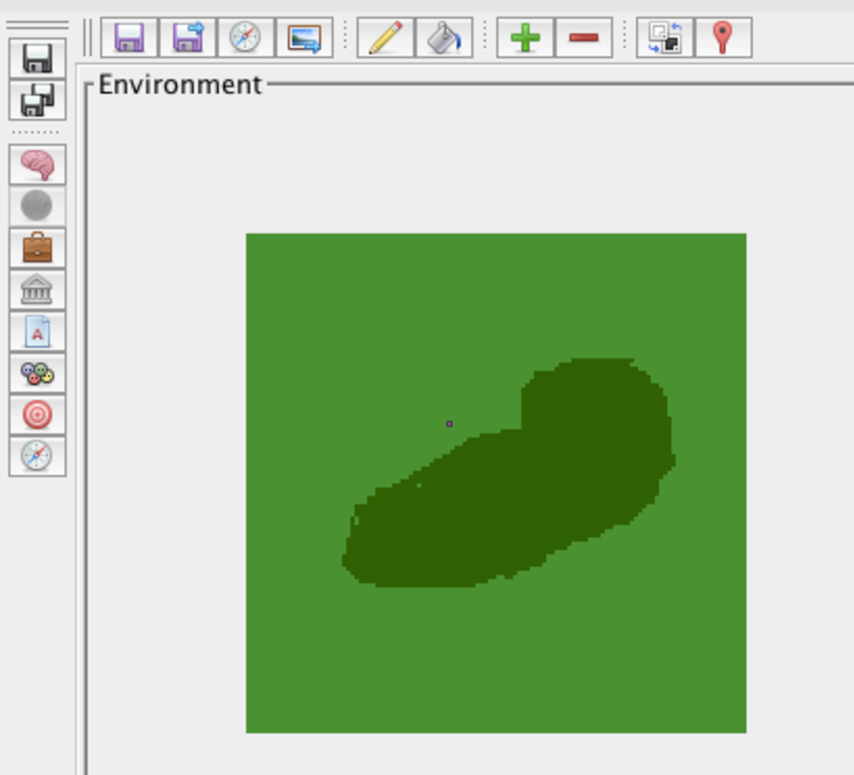
\includegraphics[scale=0.5]{locas1.pdf}
%\caption[loca]{Environnement \\}
%\label{loca}
%\end{center}
%\end{figure} 

L'inventaire des agents pourrait potentiellement comporter les objets :
\begin{itemize}
\item Boisseau\_de\_ble, objet simple ayant pour effet MangerBle qui ajoute 60 à la caractéristique Vie lorsque l'objet est utilisé et PlusBlé qui ajoute 0.1 au poids du cogniton Stock\_Ble lorsqu'on le possède, 
\item Outil, objet simple ayant pour effet PlusOutils qui ajoute 0.1 au poids du cogniton Stock\_Outils lorsqu'on le possède, 
\item Vin, objet simple ayant pour effet PlusVin qui ajoute 0.1 au poids du cogniton Stock\_Vin lorsqu'on le possède et Boire qui ajoute 40 a la caractéristique Satisfaction lorsque l'objet est utilisé.
\end{itemize}

\clearpage

\section{Cogniton, Plan, Actions}


\subsection{Cogniton}

\begin{figure}[!ht]
\begin{center}
\includegraphics[scale=0.5]{CoPl2.pdf}
\caption[CP2]{Environnement \\}
\label{CP2}
\end{center}
\end{figure} 

La figure \ref{CP2}) présente la \textit{cognition} : l'ensemble des cognitons :

\begin{itemize}
\item Compétences : Agriculteur, Viticulteur, Artisan
\item Mèmes : Base, BaseTest, DemandeBle, DemandeVin, DemandeOutil
\item Believes : EchecBle, EchecVin, Stock\_Ble, Stock\_Vin, Stock\_Outils
\item Percept : BesoinBle

\end{itemize}

\subsection{Trigger}

Le cogniton BesoinBle est conditionné par un trigger. Ce dernier permet de définir une condition, portant sur les attributs de l'agent, à l'apparition du cogniton auquel il est lié dans l'esprit de l'agent. Ainsi le cogniton BesoinBle ne sera présent dans l'esprit de l'agent 
que si la condition de son trigger est validée, c'est à dire, que si l'attribut Vie de l'agent est inférieure à la valeur 50.

\subsection{Plan, Actions}
\subsubsection{Live\_Plan}
L'arbre des actions de ce plan déployé est représenté sur la figure \ref{PL2}.
\begin{figure}[!ht]
\begin{center}
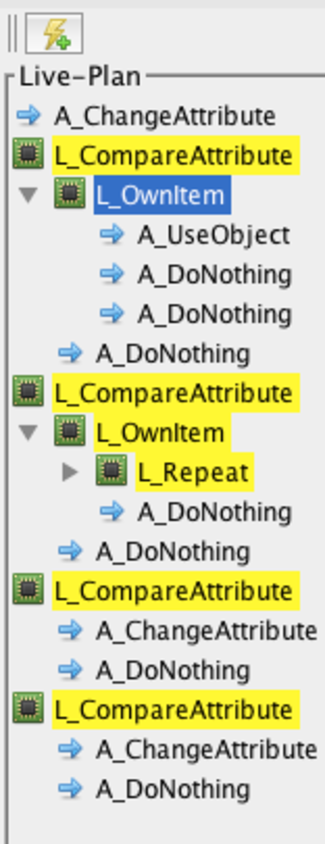
\includegraphics[scale=0.5]{LivePlan2.pdf}
\caption[PL2]{Arbre des actions du plan Live\_Plan \\}
\label{PL2}
\end{center}
\end{figure} 

Si on ouvre le fichier Live\_Plan.metaciv (dans le dossier Plans de la simulation) on accède à la description
	\begin{verbatim}

Nom : Live-Plan
Birth : false   
Self : true
Action : A_ChangeAttribute,Changed attribute(Attribute Vie),n(Integer -1)
Action : L_CompareAttribute,attributeToCompare(Attribute Vie),comparator(Comparator <),n(Double 75.0)
	Action : L_OwnItem,Object(Objet Boisseau_de_ble)
		Action : A_UseObject,Modified object(Objet Boisseau_de_ble),n(Integer 1)
		Action : A_DoNothing
		Action : A_DoNothing
	Action : A_DoNothing
Action : L_CompareAttribute,attributeToCompare(Attribute Satisfaction),comparator(Comparator <),n(Double 350.0)
	Action : L_OwnItem,Object(Objet Vin)
		Action : L_Repeat,n(Integer 1)
			Action : A_UseObject,Modified object(Objet Vin),n(Integer 1)
		Action : A_DoNothing
	Action : A_DoNothing
Action : L_CompareAttribute,attributeToCompare(Attribute Vie),comparator(Comparator <),n(Double 0.0)
	Action : A_ChangeAttribute,Changed attribute(Attribute Vie),n(Integer 1)
	Action : A_DoNothing
Action : L_CompareAttribute,attributeToCompare(Attribute Satisfaction),comparator(Comparator >),n(Double 0.0)
	Action : A_ChangeAttribute,Changed attribute(Attribute Satisfaction),n(Integer -1)
	Action : A_DoNothing
	
	\end{verbatim}	

\subsubsection{Les plans de production}
	Les plans de production de ressources (Produire du Ble et Produire de Vin) sont sensiblement identiques.
	
\begin{itemize}
\item L'agent cherche la ressource en question.
\item Si la ressource se trouve sur le patch où se trouve l'agent, ce dernier ajoute un nombre d'objets, correspondant a la ressource recherchée, fonction de la valeur du poids du cogniton de compétence relatif à ce plan.
\item Dans 10\% des cas le poids du cogniton de compétence relatif à ce plan est augmenté de 0.1 .
\item Si l'agent possède un outil celui ci est détruit.

\end{itemize}

Concernant le plan Produire des outils l'agent produit un nombre d'objets Outil fonction du cogniton de compétence relatif à ce plan et dans 10\% des cas ajoute 0.1 au poids de ce cogniton.

\subsubsection{Les plans d'échanges}
	Les plans d'échanges sont tous construits sur le même modèle. L'agent retourne tout d'abord à l'endroit où a été créé la communauté auquel il appartient, puis, se dirige vers une des autres communautés en cherchant des traces laissées par les autres agents signifiant qu'un échange a eu lieu à cet endroit. 
	
	Une fois à cet endroit, l'agent cherche autour de lui un individu souhaitant échanger l'objet que recherche l'agent, contre celui qu'il propose. Une fois la transaction faite, l'agent laisse une trace signifiant qu'un échange a eu lieu sur ce patch.

\clearpage
\section{Comportement de la simulation}
	Au début de la simulation, les agents sont crées avec la possibilité d'effectuer les plans Produire du Blé, Produire du Vin et Produire des Outils. La différenciation entre les agents va se faire au moyen de leur environnement.Leurs échecs répétés dans la production d'une ressource absente de leur environnement proche les poussant à produire une ressource présente. Une fois leurs stocks constitués les agents vont alors s'intéresser à l'échange de ressource avec une autre communauté. Les premiers à avoir des idées d'échanges seront ceux dont les terrains agricoles sont rares. Leur besoin de blé, matérialisé par le cogniton BesoinBle, les poussant à se procurer du blé, que ce soit par l'agriculture ou les échanges. Ces agents la ne possédant pas de terrains propices a l'agriculture vont alors se tourner vers l'échange. 
	
	Concernant les agents dont l'environnement est riche en terres agricoles propices a la culture du blé ne vont, quand à elles, s'intéresser aux échanges, que lorsque leur stock de blé sera suffisant pour leur garantir la survie. Les agents n'ayant pas de besoin impérieux de vin, leur préoccupation principale restera la production de blé. Les échanges et donc l'approvisionnement en vin et outils ne sera au final qu'une activité secondaire.
	
	On observe donc la création rapide de routes commerciales entre les communautés pauvres et les communauté riches en terrains agricoles motivée, tout d'abord, par le besoin de blé des communautés pauvres, puis, par la suite, par l'écoulement des stocks de blé des communautés riches. Ainsi, on observe que les premiers échanges se font a proximité des communauté riches, puis se déplacent petit a petit vers des sites équidistants des deux communautés.
\end{document}